\documentclass[12pt, oneside]{article}

\usepackage[utf8]{inputenc}
\usepackage[T1]{fontenc}
\usepackage{textcomp}
\usepackage{amsmath, amssymb}
\usepackage{fullpage}
\usepackage{graphicx}
\usepackage{amssymb, amsmath, amsthm}
\newtheorem{theorem}{Theorem}[section]
\newtheorem{corollary}{Corollary}[theorem]
\newtheorem{lemma}{Lemma}[theorem]
\title{Modeling Computer Viruses in Peer-to-Peer Networks}
\author{Abraham Porschet}
\date{\today}


% figure support
\usepackage{import}
\usepackage{xifthen}
\pdfminorversion=7
\usepackage{pdfpages}
\usepackage{transparent}

\pdfsuppresswarningpagegroup=1

\begin{document}
    \maketitle

    \section{Introduction}
        Peer to peer networks, caught on in the late 1990s and early 2000s with platforms like Limewire, Napster and MySpace. These websites
        were illustrative of the fun people could have with the internet, and also the malicious actions people could take using the internet.
        Peer to peer networks can be susceptible to various types of viruses, including self-propogating viruses such as the Samy worm \cite{VICE_2015}.\newline
        
        Obviously, the websites listed above have differences, but the main connection between them is that there are multiple users across a network
        who each have their own files or links or images publicly available for others to view or download. If a user wants to visit another user's 
        page or download another user's file(s), the user's web-client will have to connect with the other user and will then do what it was asked to do.\newline

        Some P2P networks, like Napster, have made it nearly impossibly to transmit infected files, but among other systems of the same class viruses have had a lot of success against networks like these, people can download things without being aware of it, and then viruses can download a payload to their 
        computer that adds itself to her files (so other people can download it by accident) and alters her system somehow. These viruses can behave quite similarly to 
        *actual* viruses. This means that a whole set of models, epidemiological models, are on the table to be used.\newline
        
        P2P (peer-to-peer) networks, used commercially, have millions of users that are connected in a web of millions of computer systems.
        In this web, file transfers happen rapidly, often in times much less than a second. When these webs encounter worms like the Samy worm
        or other similar viruses, they can propagate to thousands of users in very little time. If people are able to predict the spread of
        a virus inside of P2P networks, they are able to better respond to the virus at hand and better understand how to secure their network more.
        This modeling will take place in a simulation of P2P networks to assess a network's potential for propagation of viruses.\newline

        In Thommes and Coates paper on the same subject, they made the model assumption that the distribution of the infected files in the system was uniform. Essentially
        stating that each user has an equal likelihood of having an infected file, and that all users have the same expected number of infected files. However, all people are not equally
        likely to interact with infected files, or fall for internet-scams or viruses in general. In particular, the elderly have been shown to have a significantly higher risk factor for 

    \section{Methods and Model}
    
        The intent of the model is to approximate the spread of a computer virus that exists in a Peer-to-Peer (P2P) network. Note that we use the term user
        to refer to a person using a P2P client program. The term peer is used to collectively refer to a P2P client and the user directing its behaviour.
        The model examined \cite{1689197}, from Thommes and Coates, has peers of three types, Susceptible (S), Exposed (E), and Infected (I). 
    \subsection{Model}
        Since there are three different categories that a peer can fall into and each category is mutually exclusive with the others,
        it follows that at any time $t$, that  $N=S(t)+E(t)+I(t)$ where  $N$ is the number of peers in the system. We also make the assumption that the number of uninfected files is fixed at some $M$.
        The number of infected files at time  $t$ is given by a function  $K(t)$. When we then want to calculate the proportion of infected
        files to uninfected files, we get the proportion  $q(t)=\frac{K(t)}{M+K(t)}$. Thommes and Coates then assume that when a user interacts with a file,
        that it has a probability dependent on the number of infected files on the network and that the probability of an arbitrary file being infected is 
        time invariant, and is only dependent on the proportion $q(t)$, while I modeled the probability of a file being infected with a poisson distribution with
        probability mass function given by $P(K=k | \lambda) = \frac{e^{-\lambda}\lambda^k}{k!}$ where $K$ is a random variable representing the number of infected files
        infected by a peer and $k\in\mathbb{N}$ representing the number of files encountered and $\lambda(t)$ is the mean rate of of infected file encounters per minute.
        We call the function that determines this probability  $f{q(t)}$. Then, for the last introduction of new variables, we have three
        other parameters for the following three actions: a peer downloading a file from another peer, a peer executing a shared file, 
        and a peer recovering. The parameters are then,  $\lambda_S$:  the rate in files per minute at which a peer downloads new files, 
        $\lambda_E$: average rate, in files per minute, at which each peer executes files, our last rate parameter is  $\lambda_R$:
        which is the average rate of recoveries per minute, at which infected peers recover. A recovery occurs when all infected files are
        removed, returning the peer to susceptible. The state cycle of this model is  $S\to E\to I \to S\ldots$\newline

        We now derive our differential equations.
        \subsubsection{Rate at Which Infected Peers Change}
        When infected peers change back to susceptible,  $I$ decreases by 1. Recoveries occur at rate  $\lambda_R I(t)$.
        Similarly, when an exposed person executes a file, they become infected and this happens at the rate $\lambda_E E(t)$, which
        gives us our first differential equation \[
        \frac{dI(t)}{dt}=-\lambda_R I(t)+\lambda_E E(t)
        \] 
        \subsubsection{Rate at Which Exposed Peers Change}
        The rate that exposed peers decrease due to infection, is just the negative of the $E(t)$ term from the last differential equation.
        The rate at which susceptible peers are exposed is dependent on the rate at which they download files, multiplied by the probability
        that a given file is infected. This gives us a rate of \[
            \frac{dE(t)}{dt}=-\lambda_E E(t)+\lambda_S S(t)f{q(t)}
        \]
        \subsubsection{Rate at Which Susceptible Peers Change}
        This is determined by the negative of the first term of the first equation and the negative of the second term of the second equation, giving us
        \[
            \frac{dS(t)}{dt}=-\lambda_S S(t)f{q(t)}+\lambda_R I(t)
        \]
    \subsection{Results}
    Thommes and Coates did their simulations as written above with a uniform distribution while the main difference between our simulations was the probability distribution chosen.
    Since some accounts might only have infected files, existing with the goal to only infect other accounts and plenty of clean accounts, I figured that a poisson distribution
    would be a better choice for modeling the infected files per peer. Now, if we use the expectation of that distribution in order to model the spread of some 
    virus over a peer to peer network, we the formula for the probability mass function for the poisson, with
    the parameter (generally seen as $\lambda$) $q(t)$ as described in the methods section.

    When we graph the model that uses the uniform distribution and the model that uses the poisson distribution, the models actually produce much more
    similar results than expected. With the initial values given by Thommes and Coates 
    for their examples, with $\lambda_E=\lambda_S=.035$ and  $\lambda_R = .007$ and then starting in a system with 6 million files, 10,000 exposed and 1 infected peer
    we get Figures 1 and Figure 2. The probability distribution doesn't seem to have much of an effect on the equilibrium state of the system, and the two plots with
    those initial conditions and parameter values are incredibly similar.

    \begin{figure}[htbp]
        \centerline{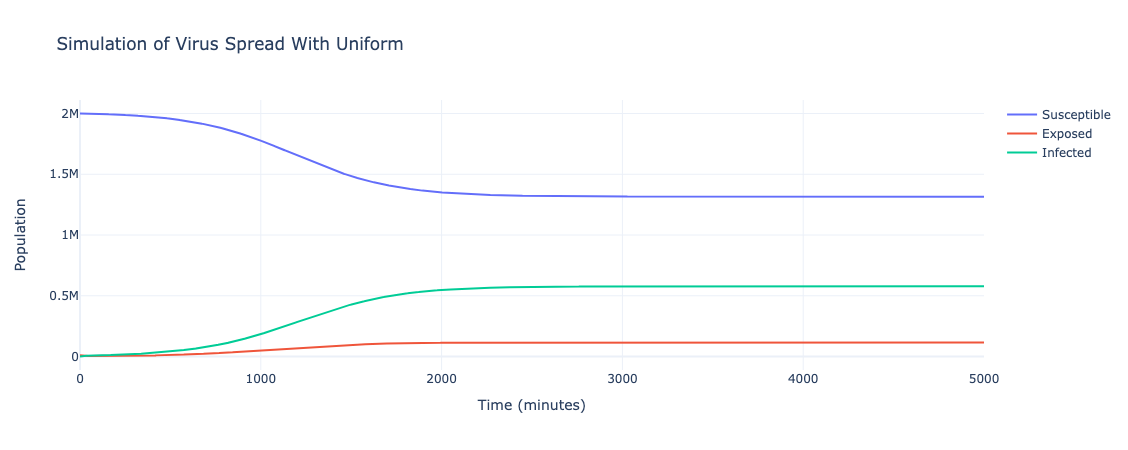
\includegraphics[scale=0.5]{Uniform(x10).png}}
        \caption{f(q(t)) as uniform distribution}
    \end{figure}
    \begin{figure}[htbp]
        \centerline{\includegraphics[scale=0.5]{Poisson(x10).png}}
        \caption{f(q(t)) as Poisson distribution}
    \end{figure}

    Now, with a radically different set of initial conditions and parameter values from the first case, you can see some slight variations between the two models. When initial conditions were chosen as
    $\lambda_E = 0.1, \lambda_S = .001,$ and $\lambda_R = .0001$ with 1000 total peers, 30 exposed and 1 infected, along with 10,000 total files. We get figures 3 and 4, which are still relatively similar,
    but have different times of intersection, where the number of exposed increases and passes the number of infected, while the number of susceptible rests at near 0 for both models.
    This behavior is a good indicator that even with small infection rates, if there is a small number of total files and a smaller number of users, it is hard to avoid
    an outcome where almost every user is either exposed to harmful files or is currently infected with malware of some kind.

    \begin{figure}[htbp]
        \centerline{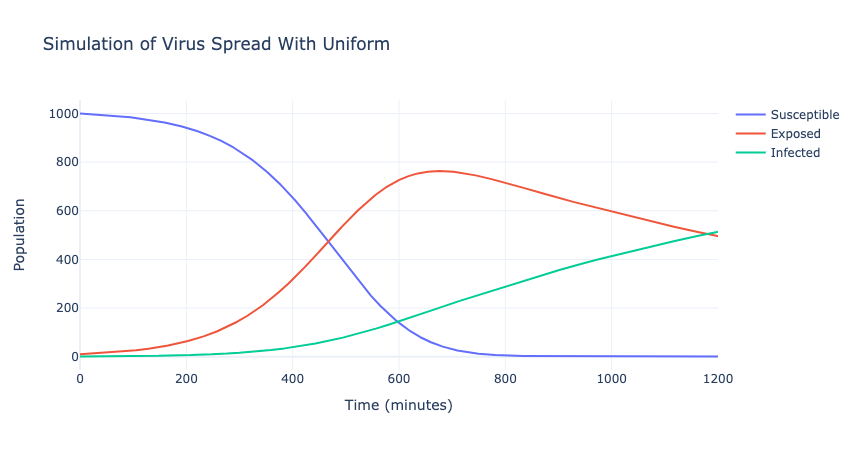
\includegraphics[scale=0.5]{Uniform(.1,.001,.0001).png}}
        \caption{f(q(t)) as uniform distribution with new parameters}
    \end{figure}
    \begin{figure}[htbp]
        \centerline{\includegraphics[scale=0.5]{Poisson(.1,.001,.0001).png}}
        \caption{f(q(t)) as Poisson distribution with new parameters}
    \end{figure}




\bibliography{paper}
\bibliographystyle{plain}
\end{document}
